In the field of linguistics and natural language processing, syntactic dependency trees are a key element for understanding the grammar of sentences and documents. These intricate hierarchical structures, with nodes representing words or tokens and edges indicating syntactic dependencies, provide valuable insights into language structure and syntax. An example can be seen in Figure \ref{fig:example_tree}. An important part of dependency tree analysis is to examine the correlation between the number of nodes (words or tokens) in the tree and the average length of its edges. This exploration can uncover significant linguistic patterns and be applied to various tasks such as machine translation, sentiment analysis, and text summarization.

\begin{figure}[!hbt]
    \centering
    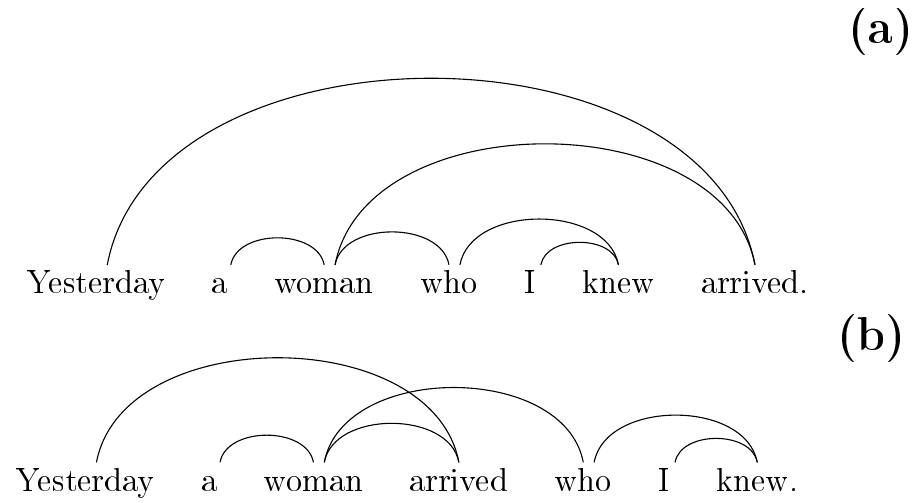
\includegraphics[width=0.5\textwidth]{figures/Screenshot_20231107_105607.png}
    \caption{Example of dependency trees. (a) A sentence without crossings. (b) An alternative ordering yielding one crossing. Extracted from \cite{Ferrer_i_Cancho_2014}}
    \label{fig:example_tree}
\end{figure}

This assignment delves into the intriguing world of dependency trees by providing collections of syntactic dependency trees from diverse languages. The primary objective is to employ non-linear regression techniques to model and understand the dependencies between the number of vertices, $n$, in a tree and the mean length, $\langle d \rangle$, of its edges.

Non-linear regression models offer a powerful toolset for addressing the complexities inherent in linguistic data. By fitting these models to our dependency tree data, we can capture and quantify the non-linear relationships that may exist between the number of vertices and the mean edge length. Throughout this assignment, we will examine various non-linear regression models, assess their suitability for the given data, and interpret the insights gained from these models.